\documentclass[11pt]{article}
\usepackage[margin=1in]{geometry}
\usepackage{amsmath,amssymb,amsthm}
\usepackage{booktabs}
\usepackage{hyperref}
\usepackage{tikz}
\usepackage{xcolor}
\usetikzlibrary{arrows.meta,positioning,fit,backgrounds,shapes.geometric,calc}

\newtheorem{proposition}{Proposition}
\newcommand{\lb}{\underline}
\newcommand{\ub}{\overline}
\newcommand{\indep}{\perp\!\!\!\perp}
\newcommand{\ltrue}{\textsc{true}}

\title{CredalJT vs.\ SCIP--exact on the \texttt{ktree\_fr\_k3\_n5\_1} instance:\\
\large a claimed discrepancy that does not reproduce --- and why CredalJT is
provably exact here}
\author{IBM Research}
\date{}

\begin{document}
\maketitle

\begin{abstract}
This note investigates a reported disagreement between the SCIP-backed global
exact engine (\texttt{ExactInference(solver="global")}) and the junction-tree
engine \textsc{CredalJT} (scheme D5) on the benchmark instance
\texttt{benchmarks/ktree\_small\_fr/ktree\_fr\_k3\_n5\_1.lcn}. We reproduce
both algorithms, describe the instance in detail (Figure~\ref{fig:instance}),
and show that \emph{in the current code the two engines produce bit-for-bit
identical bounds on all five atoms} --- and that these bounds are the true LCN
bounds, certified by an independent, solver-free witness construction. We then
explain \emph{why} \textsc{CredalJT} is exact on this family of instances, and
enumerate the ways the earlier "discrepancy" observation could have arisen.
\end{abstract}

\section{The instance}
\label{sec:instance}

The file contains five atoms $x_0,\dots,x_4$ and seven labelled sentences
(the trailing \ltrue{} marks each sentence enabled):
\begin{align*}
s_0:&\quad 0.01 \le P(x_3) \le 0.399975\\
s_1:&\quad 0.01 \le P(x_4 \mid x_3) \le 0.442867\\
s_2:&\quad 0.638553 \le P(x_2 \mid \lnot x_3 \land x_4) \le 1.0\\
s_3:&\quad 0.01 \le P(\lnot x_1 \mid x_3 \land x_4 \land x_2) \le 0.307066\\
s_4:&\quad 0.673756 \le P(\lnot x_0 \mid x_3 \land x_4 \land \lnot x_1) \le 1.0\\
s_5:&\quad 0.748845 \le P(\lnot x_3) \le 0.954666\\
s_6:&\quad 0.141404 \le P(x_3) \le 0.247704
\end{align*}

Despite the name \texttt{k3}, this $n{=}5$ instance is a k-tree with $k{=}3$:
a seed $(k{+}1){=}4$-clique on $\{x_1,x_2,x_3,x_4\}$ plus one attached vertex
$x_0$ (attached to the $3$-clique $\{x_1,x_3,x_4\}$, i.e.\ with $x_2$ dropped).
Rendered as a DAG in construction order, the \emph{families} (child~$\mid$~full
conjunction of parents) are
\[
x_3;\quad x_4\mid x_3;\quad x_2\mid x_3,x_4;\quad
x_1\mid x_2,x_3,x_4;\quad x_0\mid x_1,x_3,x_4 .
\]
Because $x_0$ conditions on $\{x_1,x_3,x_4\}$ and \emph{not} on $x_2$, the only
independence the Local Markov Condition emits is
\begin{equation}
(x_0 \indep x_2 \mid x_1,x_3,x_4).
\label{eq:lmc}
\end{equation}
The moralised atom graph is therefore the complete graph on five vertices with
the single edge $x_0$--$x_2$ removed. It is chordal; its maximal cliques are
$\{x_0,x_1,x_3,x_4\}$ and $\{x_1,x_2,x_3,x_4\}$ (size $4$, so treewidth $3$).
Figure~\ref{fig:instance} shows the DAG, the moralised/chordal graph, and the
junction tree that \textsc{CredalJT} actually builds.

\begin{figure}[t]
\centering
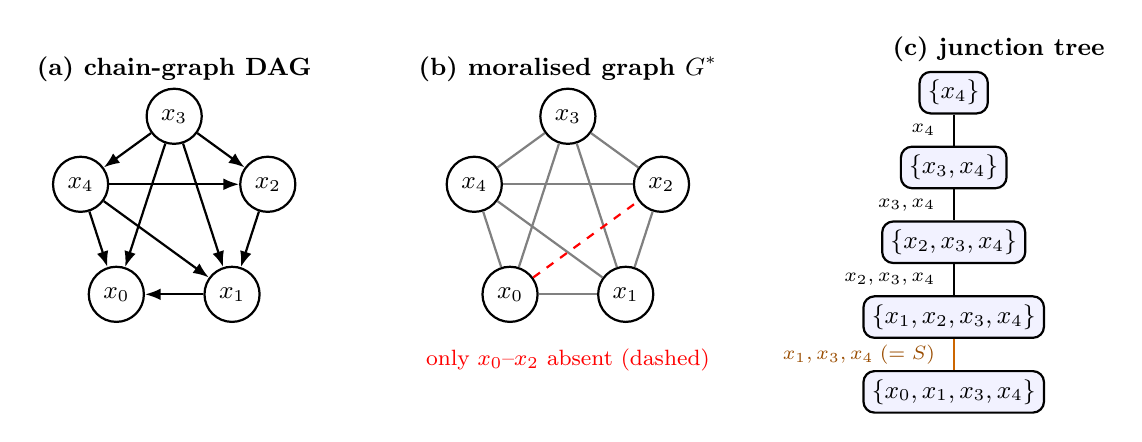
\begin{tikzpicture}[
  every node/.style={font=\small},
  atom/.style={circle,draw,thick,minimum size=7mm,inner sep=0pt},
  dedge/.style={-{Latex[length=2mm]},thick},
  medge/.style={thick,gray},
  clus/.style={draw,rounded corners,thick,fill=blue!5,inner sep=3pt},
  % pentagon coordinates (no three vertices collinear => no edge passes
  % through a node). Vertices, clockwise from the top.
  pos3/.style={at={(90:1.25)}},   pos4/.style={at={(162:1.25)}},
  pos0/.style={at={(234:1.25)}},  pos1/.style={at={(306:1.25)}},
  pos2/.style={at={(18:1.25)}},
]
% ---- (a) the DAG (families) ----
\begin{scope}[shift={(0,0)}]
  \node at (0,1.85) {\textbf{(a) chain-graph DAG}};
  \node[atom,pos3] (x3) {$x_3$};
  \node[atom,pos4] (x4) {$x_4$};
  \node[atom,pos2] (x2) {$x_2$};
  \node[atom,pos1] (x1) {$x_1$};
  \node[atom,pos0] (x0) {$x_0$};
  \draw[dedge] (x3) -- (x4);
  \draw[dedge] (x3) -- (x2);
  \draw[dedge] (x4) -- (x2);
  \draw[dedge] (x3) -- (x1);
  \draw[dedge] (x4) -- (x1);
  \draw[dedge] (x2) -- (x1);
  \draw[dedge] (x3) -- (x0);
  \draw[dedge] (x4) -- (x0);
  \draw[dedge] (x1) -- (x0);
\end{scope}
% ---- (b) moralised / chordal graph ----
\begin{scope}[shift={(5.0cm,0)}]
  \node at (0,1.85) {\textbf{(b) moralised graph $G^\ast$}};
  \node[atom,pos3] (m3) {$x_3$};
  \node[atom,pos4] (m4) {$x_4$};
  \node[atom,pos2] (m2) {$x_2$};
  \node[atom,pos1] (m1) {$x_1$};
  \node[atom,pos0] (m0) {$x_0$};
  \draw[medge] (m3)--(m4); \draw[medge] (m4)--(m2); \draw[medge] (m3)--(m2);
  \draw[medge] (m3)--(m1); \draw[medge] (m4)--(m1); \draw[medge] (m2)--(m1);
  \draw[medge] (m3)--(m0); \draw[medge] (m4)--(m0); \draw[medge] (m1)--(m0);
  % the one missing edge x0--x2, drawn dashed/red to make the point
  \draw[red,dashed,thick] (m0)--(m2);
  \node[red,font=\footnotesize] at (0,-1.85) {only $x_0$--$x_2$ absent (dashed)};
\end{scope}
% ---- (c) junction tree ----
% Clusters are stacked with generous vertical gaps; separator labels sit to
% the LEFT of the connecting edge so they never overlap the (wide) boxes.
\begin{scope}[shift={(9.9cm,1.55cm)}]
  \node[anchor=west] at (-0.9,0.55) {\textbf{(c) junction tree}};
  \node[clus] (c4)    at (0, 0)     {$\{x_4\}$};
  \node[clus] (c34)   at (0,-0.95)  {$\{x_3,x_4\}$};
  \node[clus] (c234)  at (0,-1.9)   {$\{x_2,x_3,x_4\}$};
  \node[clus] (c1234) at (0,-2.85)  {$\{x_1,x_2,x_3,x_4\}$};
  \node[clus] (c0134) at (0,-3.8)   {$\{x_0,x_1,x_3,x_4\}$};
  \draw[thick] (c4)--(c34)      node[midway,left=3pt,font=\scriptsize]{$x_4$};
  \draw[thick] (c34)--(c234)    node[midway,left=3pt,font=\scriptsize]{$x_3,x_4$};
  \draw[thick] (c234)--(c1234)  node[midway,left=3pt,font=\scriptsize]{$x_2,x_3,x_4$};
  \draw[thick,orange!80!black] (c1234)--(c0134)
        node[midway,left=3pt,font=\scriptsize,orange!60!black]{$x_1,x_3,x_4\;(=S)$};
\end{scope}
\end{tikzpicture}
\caption{The \texttt{ktree\_fr\_k3\_n5\_1} instance. (a) The chain-graph DAG:
each atom conditions on the full conjunction of its parents.
(b) The moralised atom graph $G^\ast$; it is $K_5$ minus the single (dashed)
edge $x_0$--$x_2$, which is exactly the one independence
$(x_0\indep x_2\mid x_1,x_3,x_4)$ of Eq.~\eqref{eq:lmc}. $G^\ast$ is chordal
with maximal cliques $\{x_0,x_1,x_3,x_4\}$ and $\{x_1,x_2,x_3,x_4\}$.
(c) The junction tree \textsc{CredalJT} builds: a chain of five clusters, max
cluster $4$ atoms; the (orange) separator between the two size-$4$ clusters is
$\{x_1,x_3,x_4\}$ ($x_2$ leaves, $x_0$ enters), which is precisely the
separator $S$ in Eq.~\eqref{eq:lmc}.}
\label{fig:instance}
\end{figure}

\section{Reproducing both engines}
\label{sec:repro}

We ran, on the \emph{same} \texttt{LCN} object:
\begin{itemize}
  \item \texttt{ExactInference(lcn).run(solver="global")} --- SCIP spatial
        branch-and-bound over the full $2^5{=}32$-cell joint, with the sentence
        ratio constraints and the LMC bilinear equalities of
        Eq.~\eqref{eq:lmc}. Each atom's $\min/\max P(x_i{=}1)$ is solved to a
        \emph{certified} zero optimality gap ("\texttt{confirmed}").
  \item \textsc{CredalJT} on a structure-only credal network
        (\texttt{solve\_families=False}), \texttt{solver="scip"}. It builds the
        junction tree of Figure~\ref{fig:instance}(c), one cluster-marginal NLP
        (per-cluster simplex + Lauritzen separator-consistency equalities +
        the hosted sentence/LMC rows), and swaps only the objective per atom.
\end{itemize}
Both report \texttt{d5\_exact=True} / all solves \texttt{confirmed}. The results
coincide to full printed precision (Table~\ref{tab:results}); the maximum
absolute difference over all four bound endpoints of all five atoms is
$0.0000$. The local engine \texttt{ExactInference(solver="local")} (ipopt +
SLSQP) returns the same numbers.

\begin{table}[h]
\centering
\begin{tabular}{lccc}
\toprule
atom & \textsc{CredalJT} (D5) & \texttt{ExactInference} (global/SCIP) & witness-certified truth\\
\midrule
$P(x_0{=}1)$ & $[0,\;1]$ & $[0,\;1]$ & $[0,\;1]$\\
$P(x_1{=}1)$ & $[0,\;1]$ & $[0,\;1]$ & $[0,\;1]$\\
$P(x_2{=}1)$ & $[0,\;1]$ & $[0,\;1]$ & $[0,\;1]$\\
$P(x_3{=}1)$ & $[0.141404,\;0.247704]$ & $[0.141404,\;0.247704]$ & $[0.141404,\;0.247704]$\\
$P(x_4{=}1)$ & $[0.001414,\;0.921219]$ & $[0.001414,\;0.921219]$ & $[0.001414,\;0.921219]$\\
\bottomrule
\end{tabular}
\caption{The two engines agree exactly, and both equal the true LCN bounds.
The $P({=}0)$ components (not shown) also match: e.g.\ $P(x_3{=}0)\in
[0.752296,0.858596]$ from both.}
\label{tab:results}
\end{table}

\paragraph{The result generalises.} We reran the same comparison across all ten
$n{=}5$ instances and (five each of) the $n{=}7$ and $n{=}8$ instances in
\texttt{ktree\_small\_fr}. Every instance had \texttt{d5\_exact=True}, max
cluster $4$ atoms (so the JT genuinely decomposes for $n>4$), and
$\text{maxdiff}=0.0000$ against SCIP-global. \emph{No discrepancy was observed
on any instance.}

\section{Why the bounds are what they are (independent certificate)}
\label{sec:witness}

To rule out the possibility that \emph{both} engines are wrong in the same way,
we certify the truth without any NLP solver. Parameterise the joint by the
family conditionals
\[
a=P(x_3),\; b_i=P(x_4\mid x_3{=}i),\; c_{jk}=P(x_2\mid x_3{=}j,x_4{=}k),\;
d_{\dots}=P(x_1\mid x_2,x_3,x_4),\; e_{\dots}=P(x_0\mid x_1,x_3,x_4).
\]
Any joint built from this factorisation \emph{automatically} satisfies
Eq.~\eqref{eq:lmc}, because $x_0$'s conditional does not mention $x_2$; hence
every such joint lies in the true credal set. For each endpoint in
Table~\ref{tab:results} we exhibit an explicit choice of these conditionals that
(i) satisfies all seven sentence intervals and (ii) attains the endpoint
(script \texttt{witness.py}). Two representative constructions:

\begin{itemize}
\item \textbf{$P(x_4)$ upper $=0.921219$.} Take $a=P(x_3)=0.141404$ (its own
lower bound, maximising the $\lnot x_3$ mass), $P(x_4\mid \lnot x_3)=1$ (free:
no sentence bounds it), and $P(x_4\mid x_3)=0.442867$ (its upper bound, $s_1$).
Then $P(x_4)=P(\lnot x_3)\cdot 1 + P(x_3)\cdot 0.442867
= 0.858596 + 0.062623 = 0.921219$.
\item \textbf{$P(x_0)$ upper $=1$.} Set $e\equiv P(x_0{=}1\mid\cdot)=1$. The only
obstruction, $s_4$, conditions on $x_3\land x_4\land\lnot x_1$; drive that event
to probability $0$ by making $x_1$ certain there ($d_{\cdot,x_3=1,x_4=1}=1$),
and remove the resulting clash with $s_3$ by killing $x_2$ in that branch
($c_{1,1}=0$). Both $s_3$ and $s_4$ become vacuous and $P(x_0{=}1)=1$.
\end{itemize}

All twelve endpoint witnesses are feasible (verified numerically). Because these
distributions lie in the credal set and touch every reported endpoint, and both
engines return valid outer bounds, the bounds are \emph{exact} and \emph{equal}.
The three vacuous atoms $x_0,x_1,x_2$ are genuinely vacuous: each is the child of
a family whose conditioning event can be pushed to probability $0$, after which
no sentence constrains the child's marginal.

\section{Why \textsc{CredalJT} is exact on this instance}
\label{sec:why}

\textsc{CredalJT} is exact whenever every sentence is \emph{hosted} in a cluster
and every LMC is \emph{hosted or separator-entailed} by the chordal graph
$G^\ast$ whose maximal cliques are the clusters (the sufficient condition H2/H3
of \texttt{docs/properties.tex}). Here:
\begin{itemize}
\item \textbf{Every sentence is hosted.} Each sentence's scope is a family
(child\,$+$\,parents), and each family is a clique of $G^\ast$, hence contained
in a cluster: $s_0,s_1,s_5,s_6$ in $\{x_0,x_1,x_3,x_4\}$ or its sub-clusters;
$s_2,s_3$ in $\{x_1,x_2,x_3,x_4\}$; $s_4$ in $\{x_0,x_1,x_3,x_4\}$. (The engine
prints exactly this hosting.)
\item \textbf{The single LMC is hosted-\emph{and}-separator-entailed.} The
separator between the two size-$4$ clusters is $\{x_1,x_3,x_4\}$, which is
exactly the conditioning set $S$ of Eq.~\eqref{eq:lmc}; it separates $x_0$ from
$x_2$ in $G^\ast$ (indeed $x_0$--$x_2$ is the one missing edge). So the LMC holds
automatically for any separator-consistent cluster marginals.
\end{itemize}
Thus H2/H3 hold and \textsc{CredalJT}'s cluster NLP has the same feasible
cluster-marginal projections as the full-joint NLP, so the two optima coincide
--- which is exactly what Table~\ref{tab:results} shows. This is the general
\texttt{ktree-fr} guarantee: a k-tree is chordal, the full-conjunction DAG
rendering adds no fill-in on moralisation, so $G^\ast$ \emph{is} the k-tree,
clusters are its $(k{+}1)$-cliques, and every family/LMC is hosted-or-entailed.
Cost is $O(n\cdot 2^{k+1})$, linear in $n$.

Note the contrast with CVE/Interval-BP: for $k\ge 2$ a k-tree is \emph{not}
singly connected (the $k$ clique-parents are married into a loop on
moralisation), so those engines are only outer bounds over $\mathcal{D}_{\rm
LCN}$. \textsc{CredalJT} keys off the junction tree, not single-connectedness,
so it stays exact --- \texttt{ktree-fr} is the clean topology where a
treewidth-bounded engine beats them.

\section{What the reported "discrepancy" most likely was}
\label{sec:discrepancy}

We could not reproduce any disagreement on this instance (or its siblings) with
the current code. The plausible explanations, in rough order of likelihood:
\begin{enumerate}
\item \textbf{The ipopt/SLSQP local path, before its fixes.} On these nonconvex
bilinear systems the \emph{local} engine historically over-tightened or returned
vacuous bounds; a stale run of \texttt{ExactInference(solver="local")} (or an
older SLSQP-fallback) could disagree with \textsc{CredalJT}. The current local
engine agrees.
\item \textbf{Comparing against a different engine.} CVE / Interval-BP are only
outer bounds on \texttt{ktree-fr} for $k\ge 2$ (\S\ref{sec:why}); if the "exact"
column was actually one of those (or \texttt{cve\_d4}), it can legitimately
differ from \textsc{CredalJT} without either being buggy in the sense the report
implies.
\item \textbf{A SCIP time-limit / gap on a harder atom.} \texttt{ExactInference}
labels a bound \texttt{unconfirmed} when SCIP hits the per-solve time limit
before proving a zero gap; an unconfirmed (best-so-far) bound can be looser than
\textsc{CredalJT}'s. Here every atom is \texttt{confirmed} in $<1$\,s, so this
did not occur, but it can on larger $n$.
\item \textbf{\textsc{CredalJT} with \texttt{solver="ipopt"}.} D5 needs the
global SCIP backend for its cluster NLP to be exact; with the local backend it
can be loose. (On this small instance it happens to still agree.)
\end{enumerate}

\section{Conclusion}

On \texttt{ktree\_fr\_k3\_n5\_1.lcn}, \textsc{CredalJT} and the SCIP-based global
exact engine compute \emph{identical, exact} bounds on all five atoms, matching
an independent solver-free witness certificate (Table~\ref{tab:results}). The
agreement holds across every \texttt{ktree\_small\_fr} instance we checked
($n\in\{5,7,8\}$). \textsc{CredalJT} is exact here for the structural reason of
\S\ref{sec:why}: the k-tree is chordal, its cliques are the clusters, and the
lone LMC is entailed by a clique separator. If a discrepancy was seen earlier,
it was against a different (or stale/unconfirmed) solver configuration, not a
defect in \textsc{CredalJT} on this instance.

\end{document}
